% Generated from the public primitive catalog. Original Atlas drawing; Apache-2.0.
% Target: ascon-aead; view: overview
\documentclass[border=9pt]{standalone}
% Original Atlas figure theme. Apache-2.0; see the repository LICENSE.
\usepackage[T1]{fontenc}
\usepackage{lmodern}
\usepackage{amsmath,amssymb}
\usepackage{tikz}
\usetikzlibrary{arrows.meta,positioning,calc,fit,backgrounds,decorations.pathreplacing,matrix}
\definecolor{atlasInk}{HTML}{172235}
\definecolor{atlasTeal}{HTML}{0D7B7D}
\definecolor{atlasMuted}{HTML}{637278}
\definecolor{atlasFill}{HTML}{EAF4F2}
\definecolor{atlasLine}{HTML}{B6C8C7}
\tikzset{
  every picture/.style={line width=.65pt,draw=atlasInk,>=Latex},
  every node/.style={text=atlasInk,font=\sffamily\small},
  box/.style={draw,rounded corners=1.5pt,minimum height=.9cm,minimum width=1.6cm,align=center,inner sep=6pt,fill=white},
  accent/.style={box,draw=atlasTeal,fill=atlasFill},
  wire/.style={->,line width=.7pt},
  keywire/.style={wire,draw=atlasTeal,dashed},
  xor/.style={draw,circle,fill=white,inner sep=0pt,minimum size=.38cm},
  add/.style={draw,rectangle,fill=white,inner sep=0pt,minimum size=.38cm},
  note/.style={font=\sffamily\scriptsize,text=atlasMuted,align=center},
  phase/.style={font=\sffamily\small\bfseries,text=atlasTeal},
  group/.style={draw=atlasLine,dashed,rounded corners=2pt,inner sep=8pt}
}
\newcommand{\rotl}{\mathbin{\lll}}
\newcommand{\rotr}{\mathbin{\ggg}}
\newcommand{\kx}{\operatorname{Keccak}\!\text{-}\!f[1600]}

\newcommand{\AtlasKeyBits}{128}
\newcommand{\AtlasKeyWords}{4}
\newcommand{\AtlasRounds}{N_r}
\newcommand{\AtlasPriorRounds}{N_r-1}
\newcommand{\AtlasRoundKeys}{N_r+1}
\newcommand{\AtlasDoubleRounds}{N_r/2}
\newcommand{\AtlasSixRoundGroups}{N_r/6}
\newcommand{\AtlasFLGroups}{N_r/6-1}
\newcommand{\AtlasRoundStart}{24-n}
\newcommand{\AtlasBlockBits}{b}
\newcommand{\AtlasOutputBits}{d}
\newcommand{\AtlasStateBits}{320}
\newcommand{\AtlasNonceBits}{128}
\newcommand{\AtlasCounterBits}{q}
\newcommand{\AtlasStreamBlockBits}{b}
\newcommand{\AtlasRate}{128}
\newcommand{\AtlasCapacity}{c}
\newcommand{\AtlasSteps}{N}
\newcommand{\AtlasLastStep}{N-1}
\newcommand{\AtlasWordBits}{40}
\newcommand{\AtlasHashWords}{10}
\newcommand{\AtlasFeedForward}{\boxplus}
\newcommand{\AtlasByteOrder}{big-endian}
\newcommand{\AtlasDomain}{01}
\newif\ifAtlasXof
\AtlasXoffalse
\begin{document}
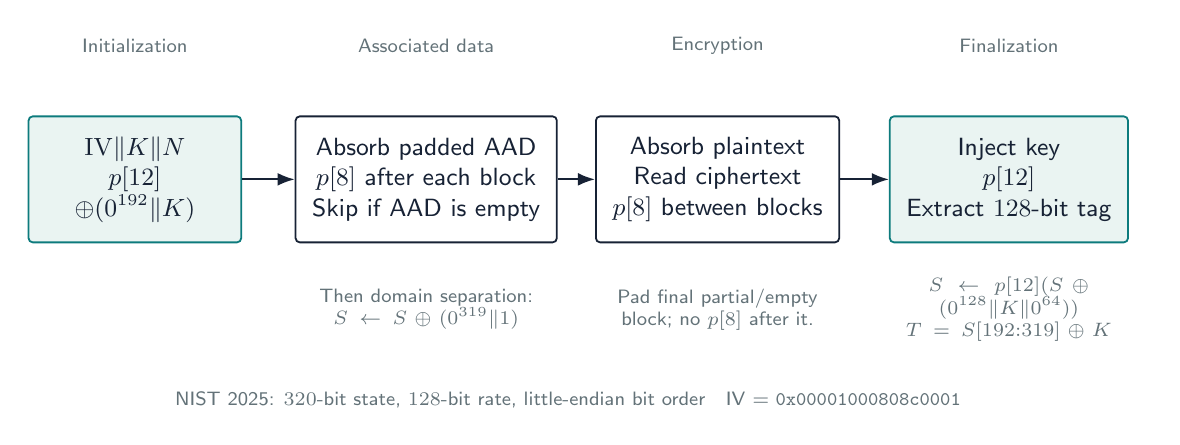
\begin{tikzpicture}
  \node[accent,minimum width=2.7cm,minimum height=1.6cm] (init) at (1,0) {$\mathrm{IV}\Vert K\Vert N$\\$p[12]$\\$\oplus(0^{192}\Vert K)$};
  \node[box,minimum width=2.7cm,minimum height=1.6cm] (ad) at (4.7,0) {Absorb padded AAD\\$p[8]$ after each block\\Skip if AAD is empty};
  \node[box,minimum width=2.7cm,minimum height=1.6cm] (msg) at (8.4,0) {Absorb plaintext\\Read ciphertext\\$p[8]$ between blocks};
  \node[accent,minimum width=2.7cm,minimum height=1.6cm] (fin) at (12.1,0) {Inject key\\$p[12]$\\Extract $128$-bit tag};
  \draw[wire] (init) -- (ad); \draw[wire] (ad) -- (msg); \draw[wire] (msg) -- (fin);
  \node[note] at (1,1.7) {Initialization}; \node[note] at (4.7,1.7) {Associated data};
  \node[note] at (8.4,1.7) {Encryption}; \node[note] at (12.1,1.7) {Finalization};
  \node[note,text width=3.2cm] at (4.7,-1.65) {Then domain separation:\\$S\gets S\oplus(0^{319}\Vert1)$};
  \node[note,text width=3.2cm] at (8.4,-1.65) {Pad final partial/empty block; no $p[8]$ after it.};
  \node[note,text width=3.4cm] at (12.1,-1.65) {$S\gets p[12](S\oplus(0^{128}\Vert K\Vert0^{64}))$\\$T=S[192{:}319]\oplus K$};
  \node[note] at (6.5,-2.8) {NIST 2025: $320$-bit state, $128$-bit rate, little-endian bit order\quad IV $=\mathtt{0x00001000808c0001}$};
\end{tikzpicture}

\end{document}
